\chapter{Algorytm wyszukiwania z tabu dla problemu układania planu zajęć}

Problem układania planu zajęć można próbować rozwiązać za pomocą algorytmu wyszukiwania z tabu. Jednak przystosowanie algorytmu do tego celu jest trudne, z uwagi na dużą złożoność problemów układania planu zajęć. Rozmiar generowanego sąsiedztwa lub stopień złożoności funkcji oceny, to tylko niektóre z nich. Poniżej omówiona została idea przystosowania algorytmu wyszukiwania z tabu do rozwiązywania problemu układania planu zajęć. Na rysunku 5.1 przedstawiono schemat przystosowanego algorytmu.

\begin{figure}
	\centering
	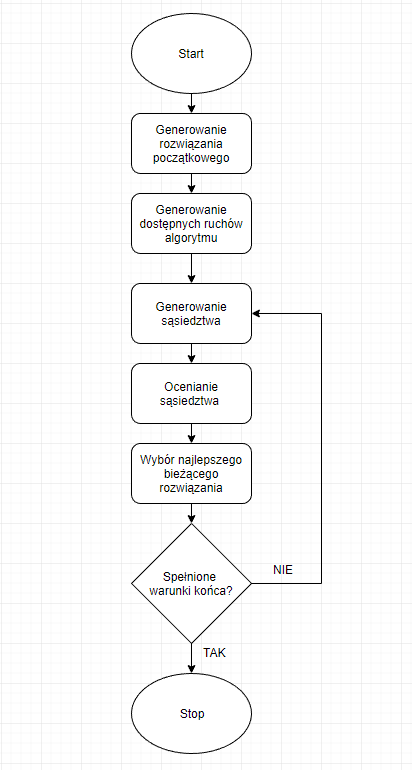
\includegraphics[height=\textheight - 1cm] {schematImplementacji}
	\caption{Schemat działania algorytmu wyszukiwania z tabu do rozwiązywania problemu układania planu zajęć.}
	\label{fig: schematImplementacji}
\end{figure}

\section{Generowanie rozwiązania początkowego}

Algorytm wyszukiwania z tabu w celu znalezienia najlepszego rozwiązania musi rozpocząć się od pewnego rozwiązania początkowego. Warto przypomnieć, że algorytm wyszukiwania z tabu jest algorytmem heurystycznym. W zależności od tego,z jakim rozwiązaniem początkowym rozpocznie on swoje działanie, może uzyskać różne rezultaty po określonej liczbie iteracji. Stworzenie początkowego planu zajęć, w którym wszystkie zajęcia rozpoczynałyby się np. w poniedziałek, w pierwszym dostępnym oknie czasowym, mogłoby spowodować znaczne wydłużenie czasu,pow którym algorytm znajdzie dostatecznie dobre rozwiązanie. Wydłużony czas wynikał by z niskiej oceny takiego planu i dłuższej ,,drogi'', jaką algorytm musi pokonać, by dojść do dobrego rozwiązania. Zdecydowano się więc na wprowadzenie elementu probabilistycznego, by zróżnicować początkowy plan zajęć. Każdemu wydarzeniu przypisywane jest losowe okno czasowe. Dobrym pomysłem byłoby zastosowanie algorytmu, który utworzył by początkowy plan zajęć z jeszcze lepszą oceną. Jednak, z uwagi na ograniczony czas implementacji, zdecydowano się pozostać przy rozwiązaniu losowym.

\section{Generowanie dostępnych ruchów algorytmu}

By ułatwić generowanie sąsiedztwa niezbędnego w dalszym działaniu algorytmu, zdecydowano się na generowanie wszystkich dostępnych ruchów dla danego kroku algorytmu. Przez ruch rozumiana jest para: wydarzenie i okno czasowe. Oznacza to, że wybranemu wydarzeniu przyporządkowane zostaje określone okno czasowe. Generowane są więc wszystkie pary, których liczba równa jest liczbie wydarzeń pomnożonej przez liczbę okien czasowych. Tak zdefiniowany ruch, może być w łatwy sposób wykorzystany podczas generacji sąsiedztwa bieżącego rozwiązania (tj. planu zajęć). Co więcej, tak wygenerowane pary nie są zależne od aktualnego rozwiązania, i dla każdego kroku algorytmu są zawsze takie same (o ile nie znajdują się na liście tabu). Dzięki temu, można łatwo reprezentować ruch jako parę indeksów i przechowywać go na liście tabu. Liczba wszystkich dostępnych ruchów określa rozmiar sąsiedztwa, które algorytm powinien przeszukać w danym kroku. Ponieważ liczba ta jest duża, konieczne było ograniczenie przeszukiwanego sąsiedztwa.

\section{Generowanie i ocenianie sąsiedztwa dla wybranego rozwiązania}

W ramach jednej iteracji, algorytm powinien wygenerować sąsiedztwo dla bieżącego rozwiązania, ocenić każdego sąsiada i wybrać najlepszego z nich. Ponieważ obliczenie funkcji oceny rozwiązania jest bardzo kosztowne, konieczne było ograniczenie rozmiaru przeszukiwanego sąsiedztwa. Rozmiar ten jest jednym z parametrów algorytmu. Po raz kolejny zdecydowano się wprowadzić element probabilistyczny. Z puli dostępnych ruchów wybierane są ruchy w sposób losowy. Każdy z wylosowanych ruchów wykonywany jest dla aktualnego rozwiązania, tworząc nowe rozwiązanie, wchodzące w skład sąsiedztwa rozwiązania aktualnego. Przykład generacji sąsiedztwa pokazano na rysunku 5.2. Tak wygenerowane sąsiedztwo jest oceniane i wybierane jest rozwiązanie najlepsze spośród dostępnych rozwiązań. Ruch, który doprowadził nas do rozwiązania najlepszego trafia na listę tabu. Następnie wybrane rozwiązanie porównywane jest z rozwiązaniem globalnie najlepszym, jakie do tej pory udało się znaleźć. Jeżeli nowe rozwiązanie jest lepsze, to staje się rozwiązaniem najlepszym globalnie. Ostatnim krokiem w ramach jednej iteracji algorytmu jest aktualizowanie listy Tabu. Dla każdego elementu aktualizowany jest czas jego trwania na liście tabu. Jeżeli jest on równy zeru, to ruch trafia z powrotem do zbioru dostępnych ruchów algorytmu.

\begin{figure}
	\centering
	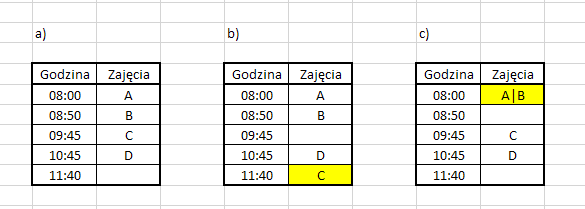
\includegraphics[width=\textwidth] {sasiedztwo}
	\caption{Przykład generacji sąsiedztwa: a) bieżące rozwiązanie, b) i c) przykładowe sąsiedztwo rozwiązania bieżącego.}
	\label{fig: sasiedztwo}
\end{figure}

\section{Funkcja oceny rozwiązania}

Najtrudniejszym elementem implementacji była funkcja oceny rozwiązania (tj. planu zajęć). Z uwagi na konieczność sprawdzania wielu warunków w stosunku do wielu elementów, jest to najbardziej czasochłonna część wykonania algorytmu. Wszystkie ograniczenia, które ma spełniać otrzymany plan zajęć muszą być badane w tej funkcji. Funkcja ta decyduje o jakości otrzymanego planu i daje duże możliwości, by w przyszłości ją udoskonalić.

Zdecydowano się wybrać do implementacji następujące ograniczenia:
\begin{itemize}
	\item przypisanie wszystkim zdarzeniom określonego czasu,
	\item unikanie konfliktów między zasobami,
	\item unikanie dzielenia zajęć trwających dłużej niż jedno okno czasowe,
	\item minimalizacja pustych okien czasowych między zdarzeniami dla grup uczniów.
\end{itemize} Każde z tych ograniczeń ma przyporządkowaną określoną wartość kary, która jest dodawana do końcowej oceny rozwiązania za każdym razem, gdy ograniczenie nie jest spełnione.

Każde zdarzenie musi mieć przypisane okno czasowe. Podczas oceny tego ograniczenia, sprawdzane są wszystkie wydarzenia. Za każdym razem, gdy któreś z wydarzeń nie będzie miało przypisanego okna czasowego, nałożona zostanie odpowiednia kara. Ograniczenie to miało zastosowanie tylko w początkowej fazie implementacji algorytmu, kiedy istniała konieczność sprawdzania poprawności wykonania algorytmu. W dalszej fazie implementacji zdecydowano, że każde zdarzenie już podczas generacji rozwiązania początkowego ma przypisane okno czasowe, a nie ma możliwości, by algorytm usunął przypisane okno czasowe. Jedynymi zmianami może być przypisanie nowego okna czasowego. Z tego powodu ograniczenie to zostało pominięte.

Ograniczenie związane z unikaniem konfliktów między zasobami sprawdzane jest w następujący sposób. Dla każdego okna czasowego wyszukiwane są wszystkie zdarzenia, które w nim występują. Konieczne jest również przeszukanie dwóch okien czasowych w tył, by sprawdzić czy nie ma tam zajęć o długości dwóch lub trzech jednostek czasu. Po znalezieniu wszystkich zdarzeń, przeszukiwane są wszystkie zasoby do nich przypisane. Każdy zasób sprawdzany jest pod kątem wystąpienia po raz kolejny w tym samym oknie czasowym. Za każde dodatkowe wystąpienie zasobu nakładana jest stosowna kara. Sprawdzanie tego ograniczenia ma największą złożoność obliczeniową, ponieważ wymaga ono wielokrotnego sprawdzania zasobów.

Ograniczenie dotyczące unikania dzielenia zajęć trwających dłużej niż jedno okno czasowe może być złamane np. w przypadku, gdy zajęcia o czasie trwania dwóch okien czasowych, przypisane są na ostatnie okno czasowe danego dnia. Wtedy druga godzina zajęć przypisana jest w pierwszym oknie czasowym dnia następnego. Oczywiście nie jest to pożądane. By wykryć złamanie tego ograniczenia konieczne jest sprawdzenie wszystkich zajęć o czasie trwania dłuższym niż jedno okno czasowe. Dla każdego z tych zajęć sprawdzane są kolejne okna czasowe występujące po nim (w zależności od długości zajęć jest to jedno lub dwa okna czasowe). Jeżeli okna czasowe przypadające na jedno zajęcie należą do różnych dni, to nakładana jest ustalona kara.

Wszystkie wyżej wymienione ograniczenia można było określić jako ograniczenia twarde. Kara za ich złamanie jest bardzo wysoka. Ostatnie ograniczenie jest ograniczeniem miękkim. Kara za jego złamanie to około 10\% wartości kary poprzednich ograniczeń. Minimalizacja pustych okien czasowych między zdarzeniami dla grup uczniów nie jest obowiązkowa aby plan był poprawny. Brak tych okien jest jednak pożądany przez uczniów. By sprawdzić to ograniczenie konieczne jest przeszukanie planu dla każdej klasy z osobna. Jeżeli dla danej klasy, w danym dniu, wystąpiły już zajęcia, a następnie wystąpiło puste okno czasowe, a po nim kolejne zajęcia, to nałożona zostanie kara. Kara jest zależna od liczby pustych okien czasowych między zajęciami.